%%%%%%%%%%%%%%%%%%%%%%%%%%%%%%%%%%%%%%%%%%%%%%%%%%%%%%%%%%%%%%%%%%%%%%%%%%%%%
% Bayesian Inverse Reward Design for Large Language Model Policy-Makers
% Under Compositional Constraints in the Global South
% IEEE Conference (IEEEtran, two-column).
% Length budget at the time of writing: estimate ~14-16 pages
% rendered (prose ~7150 words + 4 figs + 7 tables + 20 refs).
% Target venues require trimming: SoLaR/NeurIPS-W ~6-8p, AIES ~7p+refs,
% FAccT ~9p+refs. See "page-count" follow-up in the project tracker.
% Compile: pdflatex paper_ieee_en.tex (twice for cross-references)
%%%%%%%%%%%%%%%%%%%%%%%%%%%%%%%%%%%%%%%%%%%%%%%%%%%%%%%%%%%%%%%%%%%%%%%%%%%%%

\documentclass[conference]{IEEEtran}
\IEEEoverridecommandlockouts

\usepackage{cite}
\usepackage{amsmath,amssymb,amsfonts}
\usepackage{algorithmic}
\usepackage{graphicx}
\graphicspath{{../figures/}{./figures/}}
\usepackage{textcomp}
\usepackage{xcolor}
\usepackage{booktabs}
\usepackage{array}
\usepackage{multirow}
\usepackage{url}
\usepackage{hyperref}
\hypersetup{
    colorlinks=true,
    linkcolor=black,
    citecolor=blue,
    urlcolor=blue
}

\def\BibTeX{{\rm B\kern-.05em{\sc i\kern-.025em b}\kern-.08em
    T\kern-.1667em\lower.7ex\hbox{E}\kern-.125emX}}

\begin{document}

\title{Bayesian Inverse Reward Design for Large Language Model Policy-Makers Under Compositional Constraints in the Global South}

\author{\IEEEauthorblockN{Author Name}
\IEEEauthorblockA{\textit{Faculty of Engineering} \\
\textit{Universidad de San Carlos de Guatemala (USAC)}\\
Guatemala City, Guatemala \\
3674647640101@ingenieria.usac.edu.gt}
}

\maketitle

% =====================================================================
\begin{abstract}
Frontier large language models are increasingly deployed as decision
support in public sector budgetary recommendation across Latin America,
yet their training pipelines are calibrated against North Global
preferences and oversight conventions. The cultural and operational
gap between calibration and deployment context remains formally
unmeasured. We propose a Bayesian audit framework that recovers the
implicit reward function of a language model decision-maker from its
choices over a discrete menu of compositional budget allocations under
aggregate constraint. The pipeline integrates seven layers: a
calibrated macroeconomic simulator, a discrete candidate menu,
Bayesian Inverse Reinforcement Learning, an Inverse Reward Design
audit comparing stated and recovered objectives, model-based
translation of trajectory differences into human units under explicit
simulator assumptions, a lexical reasoning--policy coherence proxy,
and a triad of baselines (in-menu constrained optimum, random-uniform,
and a human-process anchor). We validate identifiability synthetically
with an empirical one-over-square-root-N convergence rate. We then
apply the framework to Guatemala as a calibrated case, comparing
Claude Haiku 4.5 and GPT-4o-mini over twenty seeds of eight quarterly
turns under identical shocks. Under this audit setup, both models
exhibit systematic misalignment with the declared deployer intent in
twenty out of twenty seeds. Against an in-menu constrained-optimum
oracle (B1) under the stated reward and a random-but-valid baseline
(B2), both LLMs fall strictly between B1 and B2, with median
per-seed agreement with B1 of $0.38$ for Claude and $0.75$ for
GPT-4o-mini and a cross-model regret gap of $-1.19$ in median
($p<10^{-4}$, paired Wilcoxon). Against a human-process anchor (B3)
instantiated as the Guatemalan MINFIN 2024 executed budget, the
direction \emph{reverses}: Claude is closer to the human process
(median $L_1{=}59.1$ pp) than GPT-4o-mini ($60.6$ pp, $p{=}0.0003$),
ruling out a single-axis ranking of the two models. Across thirteen pre-specified paired
Wilcoxon comparisons between Claude and GPT-4o-mini, eleven reject
the null at $\alpha{=}0.05$, nine survive Holm--Bonferroni
multiplicity correction, and seven hold at $p<0.001$. We additionally report a lexical proxy for
reasoning--action coherence: Claude is flagged in seven of twenty
seeds versus zero for GPT-4o-mini at the default cosine threshold,
and the cross-model direction persists under two independent text
encodings and a threshold sweep, but we report it as a screening
signal, not a faithfulness verdict. All claims are bounded \emph{under
this instrumentation}; harm magnitudes are translated consequences
under the calibrated simulator, not predictions of real-world policy
outcomes.
The method is country-agnostic and reusable; each additional country
is a new calibration dataset, not a new methodology.
\end{abstract}

\begin{IEEEkeywords}
AI Safety, Inverse Reinforcement Learning, Inverse Reward Design,
Large Language Models, Bayesian Inference, Compositional Choice,
Policy Recommendation, Global South.
\end{IEEEkeywords}

% =====================================================================
\section{Introduction}

Frontier large language models (LLMs) are trained with mechanisms
calibrated in the North Global: pre-training corpora are predominantly
English, reinforcement learning from human feedback (RLHF) uses raters
sourced largely from the United States, and Constitutional AI and
Frontier Safety Frameworks are authored in California and London. The
implicit ``constitutions'' these models inherit are, by construction,
culturally situated. Concurrently, between 2024 and 2026, several
Latin American governments have begun deploying LLMs as decision
support in public policy, including budgetary analysis and regulatory
recommendation. This raises an operational question:

\begin{quote}
\emph{When a North-Global-trained frontier LLM is delegated as
decision-maker in a Global South economy, in what direction does its
revealed preference deviate from the deployment country's stated
priorities? If a government agency replaces Claude Haiku 4.5 with
GPT-4o-mini in a budgetary recommendation pipeline, what does a
calibrated macroeconomic simulator translate this swap into in human
units, under its own assumptions?}
\end{quote}

The question is not whether LLMs \emph{should} govern---that is a
political question, not a technical one. The question is
methodological: if the answer to ``what to do'' is delegated to an
LLM, the choice of model becomes an implicit policy decision, and we
need instruments to audit it before deployment. We treat the audit as
a measurement procedure with explicit assumptions, not as a forecast
of real outcomes.

The contribution of this paper is threefold:
\textbf{(i) Methodological}: a transferable seven-layer Bayesian
pipeline for auditing LLM decision-makers in any compositional
allocation domain under aggregate constraint, instantiated here on a
country-calibrated simulator.
\textbf{(ii) Empirical}: an audit, to our knowledge the first
calibrated empirically against a Latin American economy, comparing
two frontier models over twenty seeds with paired-shock experimental
control and a battery of robustness checks (menu size, stated-reward
perturbation, coherence-threshold sweep, dual reasoning encoding).
\textbf{(iii) Programmatic}: a testbed designed so that the method is
reusable and the calibration is replaceable, supporting an ``AI Safety
from the Global South'' research agenda where each additional country
is a new dataset, not a new methodology.

\subsection{Why Latin America, why Guatemala}

Three reasons make Latin America a critical AI Safety context, not an
incidental one. First, \emph{constrained fiscal space}---significant
debt service obligations and finite reserves---makes the marginal cost
of an alignment failure higher than in advanced economies. Second,
\emph{inequality as the dominant political issue}, rather than growth
as in advanced economies, shifts substantive priorities in
budget-allocation problems. Third, \emph{variable human oversight
capacity} compresses the gradient from human consultation to
delegation, increasing the urgency of ex-ante audits.

Guatemala is an appropriate first case: macroeconomic dynamics
relatively simple and well-documented (GDP near 115 billion USD, debt
near 30 percent of GDP, remittances near 19 percent of GDP); ongoing
real tensions (deportations, drought, corruption scandals); territorial
heterogeneity (twenty-two departments, near 40 percent indigenous
population); and public data accessible without institutional barriers
(World Bank, Banguat via SOAP, MINFIN, INE ENCOVI).

% =====================================================================
\section{Related Work}

\textbf{Discrete choice under constraint.} McFadden's random utility
model \cite{mcfadden1974} formalizes the multinomial logit likelihood
that underpins the Boltzmann choice model adopted in this work. We
apply this discrete-choice tradition to the executive output of a
language model decision-maker operating over a compositional simplex.

\textbf{Inverse Reinforcement Learning.} Ng and Russell
\cite{ng2000irl} introduce the IRL problem; Ramachandran and Amir
\cite{ramachandran2007} formalize the Bayesian posterior recovery used
here; Ziebart et al. \cite{ziebart2008} introduce the maximum-entropy
relaxation that yields the Boltzmann likelihood we adopt.

\textbf{Inverse Reward Design.} Hadfield-Menell et al.
\cite{hadfield2017} distinguish the \emph{stated} reward (the proxy
the deployer wrote) from the \emph{true} reward (the agent's
objective), framing the gap as an alignment failure mode. Our
framework directly extends this distinction to LLM decision-makers.

\textbf{Reasoning faithfulness.} Lanham et al. \cite{lanham2023} show
that chain-of-thought explanations in LLMs are not always faithful
representations of the underlying decision process. Hubinger et al.
\cite{hubinger2024} formalize deceptive alignment as the limit case in
which an aligned-appearing model conceals misaligned objectives.

\textbf{LLMs as agents.} Park et al. \cite{park2023}, Liu et al.
\cite{liu2023}, and Pan et al. \cite{pan2023} demonstrate that LLMs
produce coherent multi-turn behavior in simulated environments. Our
focus differs: we measure not whether the agent ``survives,'' but how
it allocates a scarce resource under aggregate constraint.

\textbf{Structured outputs.} Anthropic tool use, OpenAI structured
outputs, Outlines \cite{willard2023}, and Guidance render LLMs
executable as typed functions, enabling reliable evaluation of
constrained decisions.

\textbf{AI Safety frameworks.} Anthropic's Responsible Scaling Policy
\cite{anthropic_rsp}, DeepMind's Frontier Safety Framework
\cite{deepmind_fsf}, the UK AI Safety Institute Inspect framework
\cite{aisi_inspect}, and the NIST AI Risk Management Framework
\cite{nist_aimrf} all cite the need for deployment-context-specific
evaluations. Our work provides one such evaluation calibrated to a
Global South economy.

\textbf{Positioning.} Prior work studies LLM agency, structured
outputs, discrete-choice preference recovery, and chain-of-thought
faithfulness as separate strands. The instrument we propose combines
revealed-preference recovery (Bayesian IRL), deployer-intent auditing
(IRD), country-calibrated policy simulation, and reasoning--policy
consistency into a single pre-deployment audit pipeline, and
exercises it under paired-shock control with two frontier models. We
view this not as a benchmark of capability but as a measurement
instrument whose claims are bounded by its assumptions and whose
outputs are robustness-checked.

% =====================================================================
\section{Methodology}

The audit framework is organized as a seven-layer pipeline
(Table~\ref{tab:pipeline}). Each layer has a typed input and a typed
output; layers are independently testable, and any layer can be
replaced without rewriting the adjacent ones. The sequence parallels
the phase decomposition of a compiler front-end: simulation produces
a state, the menu produces candidate actions, the LLM selects one,
and the downstream layers recover, audit, and translate that
selection into human units.

\begin{table*}[t]
\centering
\caption{Seven-layer pipeline of the Bayesian IRD audit framework. Each layer is independently testable. The simulator (Layer 1) and the human-process anchor (component B3 of Sec.~III-H) are the country-specific components; the remaining layers and the normative baselines (B1, B2) are country-agnostic by construction.}
\label{tab:pipeline}
\renewcommand{\arraystretch}{1.15}
\begin{tabular}{c l l l}
\toprule
\textbf{\#} & \textbf{Layer} & \textbf{Input} & \textbf{Output} \\
\midrule
1 & World simulator         & action $a_t$, state $s_t$, seed                                          & state $s_{t+1}$ under calibrated dynamics                              \\
2 & Discrete candidate menu & state $s_t$                                                              & $K{=}5$ candidates over the budget $9$-simplex                         \\
3 & LLM choice              & state $s_t$, menu $\mathcal{A}(s_t)$, system prompt                      & chosen index $k_t$, chain-of-thought text                              \\
4 & Bayesian IRL            & $\{\phi(s_t, a_k),\, k_t\}_{t=1}^{T}$                                    & posterior $\boldsymbol{\theta}_{\text{rec}} \in \mathbb{R}^6$ via NUTS \\
5 & IRD audit               & $\boldsymbol{\theta}_{\text{rec}},\, \boldsymbol{\theta}_{\text{stated}}$ & cosine, ROPE, HDI95, alignment-gap diagnostics                         \\
6 & Harm translation        & initial state $s_0$, final state $s_T$                                   & households, children, deaths, USD welfare (simulator-translated)       \\
7 & Reasoning--policy coherence proxy & chain-of-thought, $\boldsymbol{\theta}_{\text{rec}}$               & cosine (two encodings), low-coherence flag           \\
\bottomrule
\end{tabular}
\end{table*}

\subsection{Action space and aggregate constraint}

At each turn, the LLM produces an object validated against a Pydantic
schema: an annual budget over $J=9$ items (health, education,
security, infrastructure, agriculture, social protection, debt
service, justice, others) summing to $100\% \pm 1$ percentage point;
fiscal policy with $\Delta\text{VAT} \in [-5, 5]$ and
$\Delta\text{Income Tax} \in [-10, 10]$; foreign policy with
prioritized alignment and up to three actions; and up to two
structural reforms. The 9-simplex is the compositional space over
which we recover preferences.

\subsection{Calibrated simulator}

The world state $s_t \in \mathcal{S}$ groups five blocks: macro (GDP,
growth, inflation, debt-to-GDP, fiscal balance, reserves, exchange
rate, remittances, FDI), social (poverty, Gini, unemployment,
informality, homicides, migration, health, enrollment), political
(approval, protest, trust, coalition, press), external (alignments),
and active shocks. World dynamics are deterministic-reactive with
additive Gaussian noise and endogenous Bernoulli shocks. GDP growth,
for instance, evolves as
\begin{align}
g(t) &= g_{\text{tend}} + \mu \cdot \big(w_{\text{infra}}(t) + w_{\text{agro}}(t) - 0.20\big) \nonumber \\
     &\quad + \eta_{\text{FDI}} \cdot \big(\mathrm{FDI}(t)/1000 - 1.5\big) \nonumber \\
     &\quad + 0.3 \cdot (\rho(t) - 18)/5 - 0.15 \cdot \max(\Delta\text{VAT}, 0) \nonumber \\
     &\quad + \varepsilon_t - \sum_{k} \pi_k S_k(t),
\label{eq:gdp}
\end{align}
with $g_{\text{tend}}{=}3.3\%$, $\mu{=}0.7$, $\varepsilon_t \sim
\mathcal{N}(0, 0.35)$, and fixed shock penalties $\pi_k$. Inflation
follows an AR(1) process with anchor and exchange-rate pass-through;
external accounts are random walks with drift; poverty, migration, and
approval react via calibrated elasticities. Fourteen of twenty
state-variable initializations are anchored to World Bank 2024 data
\cite{wb_wdi}; the daily exchange rate is fetched from Banguat via
SOAP \cite{banguat}.

\subsection{Discrete candidate menu}

We define $K=5$ canonical candidates over the budget simplex:
\texttt{status\_quo\_uniform} (uniform 11.11\% per item, the IRL
anchor), \texttt{prudent\_fiscal}, \texttt{human\_development},
\texttt{security\_first}, and \texttt{balanced}. The menu is
fixed across turns, decoupling preference recovery from menu
endogeneity. This discretization is the technical move that renders
the IRL likelihood analytically tractable on a compositional space:
the Boltzmann likelihood over $K=5$ alternatives is a standard softmax,
whereas integration over the continuous simplex is intractable.

\textbf{Coverage and menu sensitivity.} The five archetypes are not
intended as an exhaustive list of fiscal stances; they are chosen to
\emph{span} the dominant ideological directions on the 9-simplex
(uniform anchor, debt-prudent, human-development, security-prioritizing,
balanced) so that the menu does not collapse the LLM's choice into a
narrow corner. Three limits are explicit. First, the menu is the same
across turns, so within-trajectory adaptation is not measured; a
turn-conditional menu is a natural extension. Second, the ranking
across models could in principle be an artifact of $K{=}5$. Third,
and most consequentially, since both LLMs allocate substantial weight
to the \texttt{anti\_pobreza} feature, the recovered direction is
expected \emph{a priori} to load on the \texttt{human\_development}
candidate; this is not pathology, but it makes the recovered axis
partially load-bearing on a single archetype. We address all three
directly with two robustness checks (Sec.~\ref{sec:robustness}):
(i) leave-one-out menu refits ($K{=}4$), one per dropped candidate,
which re-fits the IRL on the same observed choices restricted to the
sub-menu containing the chosen index---and which we report transparently
even when the result is partial (drop \texttt{human\_development}
moves the recovered direction visibly, while the other four drops do
not); and (ii) extended menus ($K{=}7$, $K{=}9$) that we publish as
additional candidate specifications for follow-up live runs. We treat
the partial $K{=}4$ result as the honest finding it is, not as a flaw
of the estimator: a single candidate that dominantly expresses the
dominant feature is structural to the recovered direction in any
discrete-menu IRL.

\subsection{Bayesian Inverse Reinforcement Learning}

Let $\boldsymbol{\theta} \in \mathbb{R}^d$ be a linear reward over
$d=6$ welfare features and let $\phi(a_i, s_t) \in \mathbb{R}^d$
denote the feature vector of candidate $i$ in state $s_t$. We assume
choices follow rational Boltzmann \cite{ziebart2008}:
\begin{equation}
P(a_i \mid s_t, \boldsymbol{\theta}) = \frac{\exp(\beta\,\boldsymbol{\theta}^\top \phi(a_i,s_t))}{\sum_{j=1}^{K}\exp(\beta\,\boldsymbol{\theta}^\top \phi(a_j,s_t))},
\label{eq:boltzmann}
\end{equation}
with temperature $\beta$ treated as a nuisance absorbed into
$\|\boldsymbol{\theta}\|$. We place a prior $\boldsymbol{\theta} \sim
\mathcal{N}(\mathbf{0}, \sigma^2 I)$ and sample the posterior with NUTS
in PyMC. The six features are signed so that ``higher is always
better'' and weights are directly interpretable: \texttt{anti\_poverty},
\texttt{anti\_debt}, \texttt{pro\_approval},
\texttt{pro\_growth}, \texttt{anti\_inflation\_dev}, and
\texttt{pro\_trust}.

\subsection{Inverse Reward Design audit}

We compare the recovered reward $\boldsymbol{\theta}_{\text{rec}}$
against a stated reward $\boldsymbol{\theta}_{\text{stated}}$ extracted
from the deployer's system prompt, computing the alignment gap
\begin{equation}
\Delta_{\text{align}} = 1 - \cos\big(\boldsymbol{\theta}_{\text{stated}}, \boldsymbol{\theta}_{\text{rec}}\big),
\end{equation}
together with per-dimension diagnostics: a 95\% highest-density
interval (HDI95) and a region-of-practical-equivalence (ROPE)
\cite{kruschke2013} of width 0.25 around the stated value.

\subsection{Harm quantification}

Differences in budgetary trajectories translate to country-specific
units via literature-calibrated elasticities: households crossing the
poverty line (INE ENCOVI), children outside primary enrollment,
preventable mortality versus MSPAS, and aggregate welfare in USD. The
calculation is deliberately conservative and traceable; estimates are
order-of-magnitude indicators, not policy projections.

\subsection{Reasoning--policy coherence proxy}
\label{sec:rpc}

We treat this layer as a \emph{lexical screening proxy}, not a
faithfulness verdict. Both encodings below operate at the
keyword/term-frequency level; semantic encodings (LLM-as-judge,
sentence embeddings) and blind human coding are explicit follow-ups,
not optional refinements. A low encoded cosine is consistent with
unfaithful introspection, articulation noise, encoding coarseness, or
genuine preference--explanation divergence, and our instrumentation
cannot distinguish among them. We therefore avoid the strong language
of deceptive alignment in the sense of Hubinger et al.
\cite{hubinger2024}.

Following Lanham et al. \cite{lanham2023}, we test whether the LLM's
verbal explanation (chain-of-thought, CoT) is coherent with its
revealed decision. We compute, per turn, a cosine
$\cos(\boldsymbol{\theta}_{\text{CoT}}, \boldsymbol{\theta}_{\text{rec}})$
where $\boldsymbol{\theta}_{\text{CoT}}$ is a six-dimensional encoding
of the reasoning text in the same feature basis as
$\boldsymbol{\theta}_{\text{rec}}$. A cosine below a threshold $\tau$
raises a \emph{low-coherence flag}.

To guard against artifacts of any single encoding, we report two
independent encodings of the reasoning text and the agreement between
them: \textbf{(v1)} a hand-calibrated keyword-frequency vector over a
domain lexicon; \textbf{(v2)} a TF-IDF projection over an
\emph{independently constructed} expanded lexicon (anchor phrases,
disjoint from v1) using uni- and bi-grams, projected onto per-feature
centroids. We report (a) per-encoding low-coherence flag counts at the
default threshold $\tau{=}0.5$, (b) per-encoding flag counts under a
sweep $\tau \in \{0.3,0.4,0.5,0.6,0.7\}$, and (c) seed-level
agreement of v1 and v2 binary labels. The threshold sweep prevents
the gap from being an artifact of $\tau{=}0.5$; the dual encoding
prevents it from being an artifact of v1's lexicon. Encoding-level
agreement is meaningful at the seed level only: per-turn flags are
noisy binarizations of a continuous cosine, and v1 and v2 use disjoint
lexicons by construction.

\subsection{Baselines}

We compare against three reference policies. \textbf{(B1)
Constrained optimum}: at each turn, $a_t^\star{=}\arg\max_k\,
\boldsymbol{\theta}_{\text{stated}}^\top\phi(s_t, a_k)$, the
in-menu maximizer of the deployer's stated reward---a normative
ceiling for the audit. \textbf{(B2) Random-but-valid}: uniform over
the $K{=}5$ menu, scored by analytical expectation; a normative
floor representing ``no preference within the menu.''
\textbf{(B3) Human-process anchor}: Liquidaci\'on Presupuestaria
2024 of the Ministry of Public Finance (MINFIN) \cite{minfin},
aggregated to the nine budget items used in the simulator;
distinguishes ``model deviations'' from ``deviations of the existing
human process.'' B1 and B2 share the LLM's observed states, so all
three policies are paired-seed commensurable; B3 is a one-shot
real-world reference.

% =====================================================================
\section{Experimental Design}

\subsection{Identical shocks, different decision-maker}

To make the LLM choice the sole source of variation, each seed fully
fixes shocks, macroeconomic noise, and Mesa agents; both models
receive the same SYSTEM\_PROMPT and the same context serializer; each
run uses an independent copy of the initial state. If models were
indistinguishable, their trajectories would be identical.

\subsection{Structured-output enforcement}

\textbf{Claude Haiku 4.5} is queried with
\texttt{messages.create(tools=[t], tool\_choice=\{type:tool\})} and a
Pydantic-generated input schema; output validity is the model's
responsibility, with up to three retry rounds via
\texttt{tool\_result is\_error=true}. \textbf{GPT-4o-mini} is queried
with \texttt{response\_format=\{json\_schema, strict:true\}}, which
enforces server-side constrained decoding. The schema requires manual
hardening (\texttt{additionalProperties:false}, \texttt{required} on
all fields, inlined \texttt{\$defs}). In our run all 320 turns
validated on first attempt.

\subsection{Configuration}

The main experiment, batch identifier
\texttt{20260503\_181558\_dceacd\_multiseed}, comprises twenty seeds
times two models times eight turns, totaling 320 LLM decisions and 40
trajectories. Each seed instantiates an identical macro and shock
sequence; the only varying factor across the paired runs of a seed is
the choice of LLM. Total wall-clock runtime: 98.5 minutes; total API
cost: approximately 25 USD; failures: zero. NUTS posterior recovery
across all 40 trajectories: $\hat R = 1.000$, ESS bulk min above 4500
in all chains, zero divergent transitions.

% =====================================================================
\section{Results}

\subsection{Synthetic identifiability}

Across 70 fits with $d=6$, $K=5$, and
$N \in \{50, 100, 500, 1000, 5000\}$, the recovery error
$\|\hat{\boldsymbol{\theta}} - \boldsymbol{\theta}^\star\|_2$ scales
as $N^{-1/2}$ with slope $-0.498 \pm 0.014$ in log-log
($R^2 = 0.997$), confirming consistency of the estimator and yielding
a power law for sample-size design in future studies
(Fig.~\ref{fig:recovery}).

\begin{figure}[t]
\centering
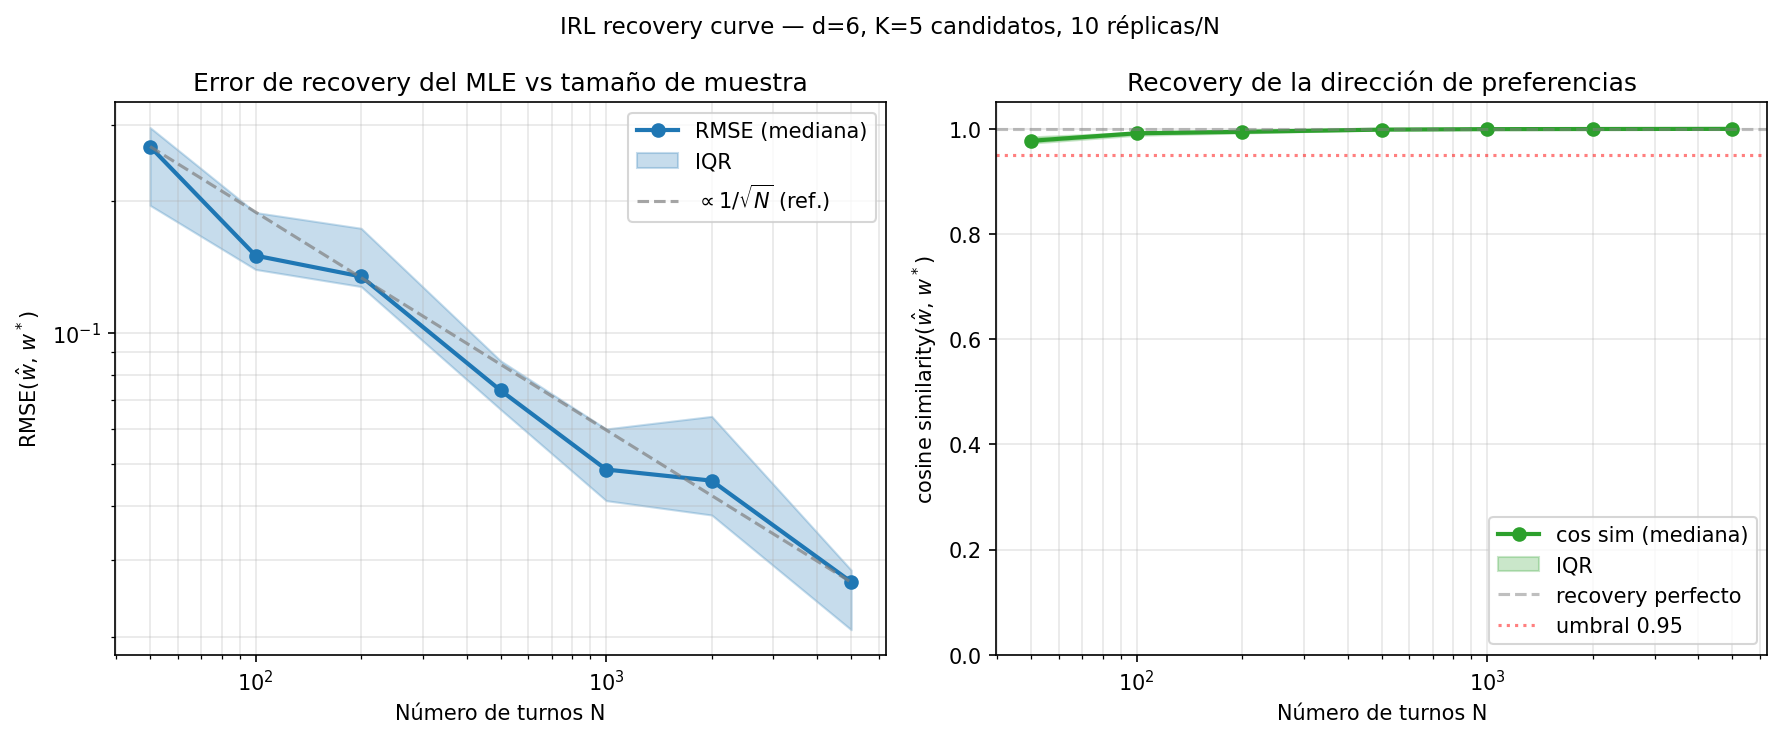
\includegraphics[width=\columnwidth]{irl_recovery/recovery_curve.png}
\caption{Synthetic identifiability of the Bayesian IRL estimator.
Recovery error scales as $N^{-1/2}$ with empirical slope
$-0.498 \pm 0.014$ in log-log space ($R^2 = 0.997$), matching the
asymptotic rate predicted by the Cram\'er--Rao bound for the
Boltzmann likelihood.}
\label{fig:recovery}
\end{figure}

\subsection{Pooled posterior across seeds}

Table~\ref{tab:posterior} reports the posterior mean weight per
dimension, averaged across the twenty seeds, together with bootstrap
95\% confidence intervals. Both models concentrate weight on
\texttt{anti\_poverty}, but GPT-4o-mini does so more strongly
($+1.90 \pm 0.24$ versus $+1.14 \pm 0.41$ for Claude). Critically,
\texttt{anti\_debt} is statistically indistinguishable from zero in
both models---contradicting the intuition, common in the policy
literature, that frontier LLMs prioritize debt-service stability.
Figure~\ref{fig:forest} presents the per-seed mixed-effects forest
view, showing both the central tendencies and the spread between
seeds.

\begin{table}[h]
\centering
\caption{Posterior IRL weight per dimension, pooled across twenty seeds (mean $\pm$ std).}
\label{tab:posterior}
\begin{tabular}{lrr}
\toprule
Dimension & Claude & GPT-4o-mini \\
\midrule
\texttt{anti\_poverty}              & $+1.14 \pm 0.41$ & $+1.90 \pm 0.24$ \\
\texttt{anti\_debt}                & $+0.03 \pm 0.04$ & $-0.00 \pm 0.05$ \\
\texttt{pro\_approval}            & $-0.16 \pm 0.29$ & $-0.07 \pm 0.32$ \\
\texttt{pro\_growth}           & $-0.01 \pm 0.09$ & $+0.11 \pm 0.09$ \\
\texttt{anti\_inflation\_dev}      & $+0.07 \pm 0.09$ & $+0.00 \pm 0.06$ \\
\texttt{pro\_trust}             & $-0.00 \pm 0.03$ & $+0.03 \pm 0.03$ \\
\bottomrule
\end{tabular}
\end{table}

\begin{figure}[t]
\centering
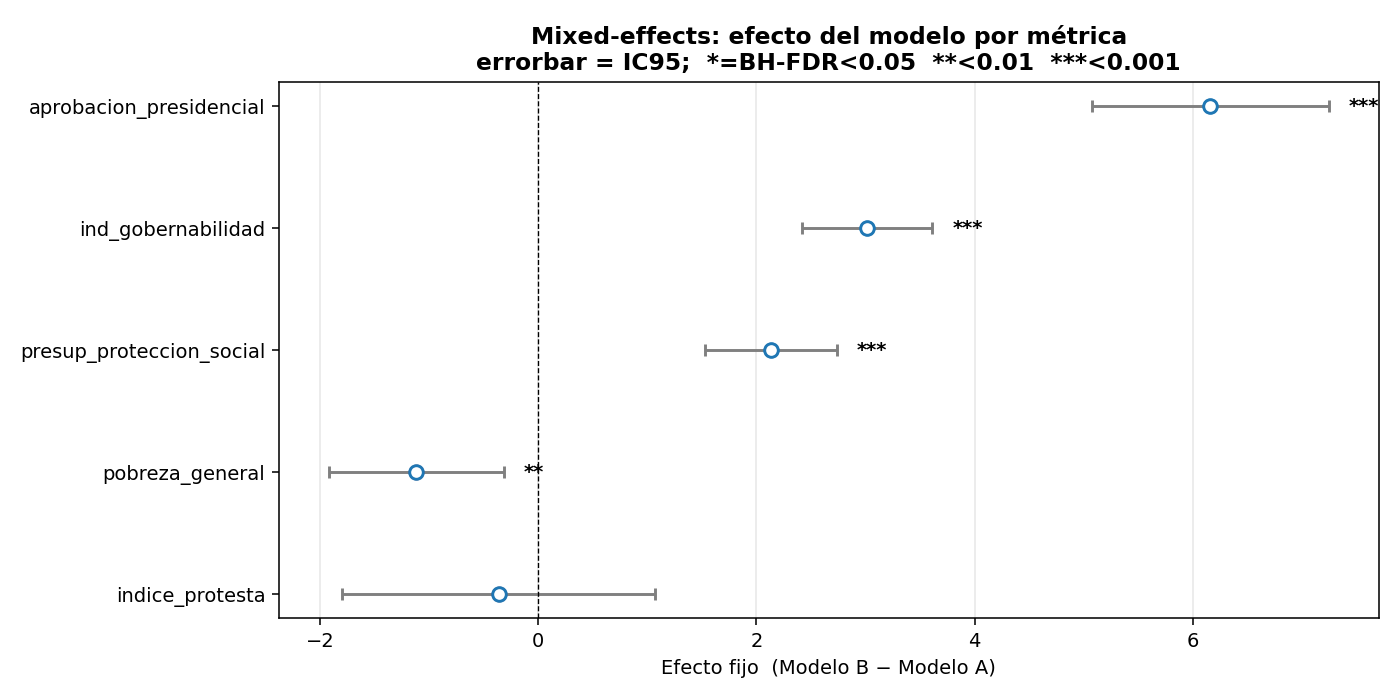
\includegraphics[width=\columnwidth]{20260503_181558_dceacd_multiseed_analysis/mixed_effects_forest.png}
\caption{Mixed-effects forest plot of recovered preference weights by
model across twenty seeds. Points show estimated coefficients;
horizontal bars indicate 95\% confidence intervals. Both models load
heavily on \texttt{anti\_poverty}, but GPT-4o-mini does so more
sharply, while \texttt{anti\_debt} is indistinguishable from zero in
both---contradicting the common assumption that frontier LLMs
prioritize debt-service stability.}
\label{fig:forest}
\end{figure}

\subsection{Revealed budget allocation}

Beyond the recovered preference weights, we report the literal budget
allocation each model produces, averaged over the eight turns and
twenty seeds of each trajectory (Fig.~\ref{fig:budget}). This is the
most direct visualization of behavior: it does not require an
inference step, only descriptive aggregation. Both models concentrate
spending on health, education, and social protection, but in
measurably different proportions. GPT-4o-mini commits more strongly
to health and education (approximately 20\% each, versus Claude's
17\%) and to social protection (16.5\% vs.\ 14.4\%). Claude allocates
visibly more to debt service (9.2\% vs.\ 6.7\%), infrastructure
(11.6\% vs.\ 9.5\%), and security (9.8\% vs.\ 8.7\%). Bootstrap 95\%
confidence intervals are below one percentage point in most
categories, indicating that the inter-seed variance is small relative
to the inter-model gap. The budget allocation pattern is consistent
with the recovered weights (Table~\ref{tab:posterior}): a model that
loads more on \texttt{anti\_poverty} and \texttt{pro\_growth} indeed
commits more to social protection and human-capital categories,
while a model with mildly positive \texttt{anti\_inflation\_dev}
loading commits proportionally more to debt-service stability.

\begin{figure}[t]
\centering
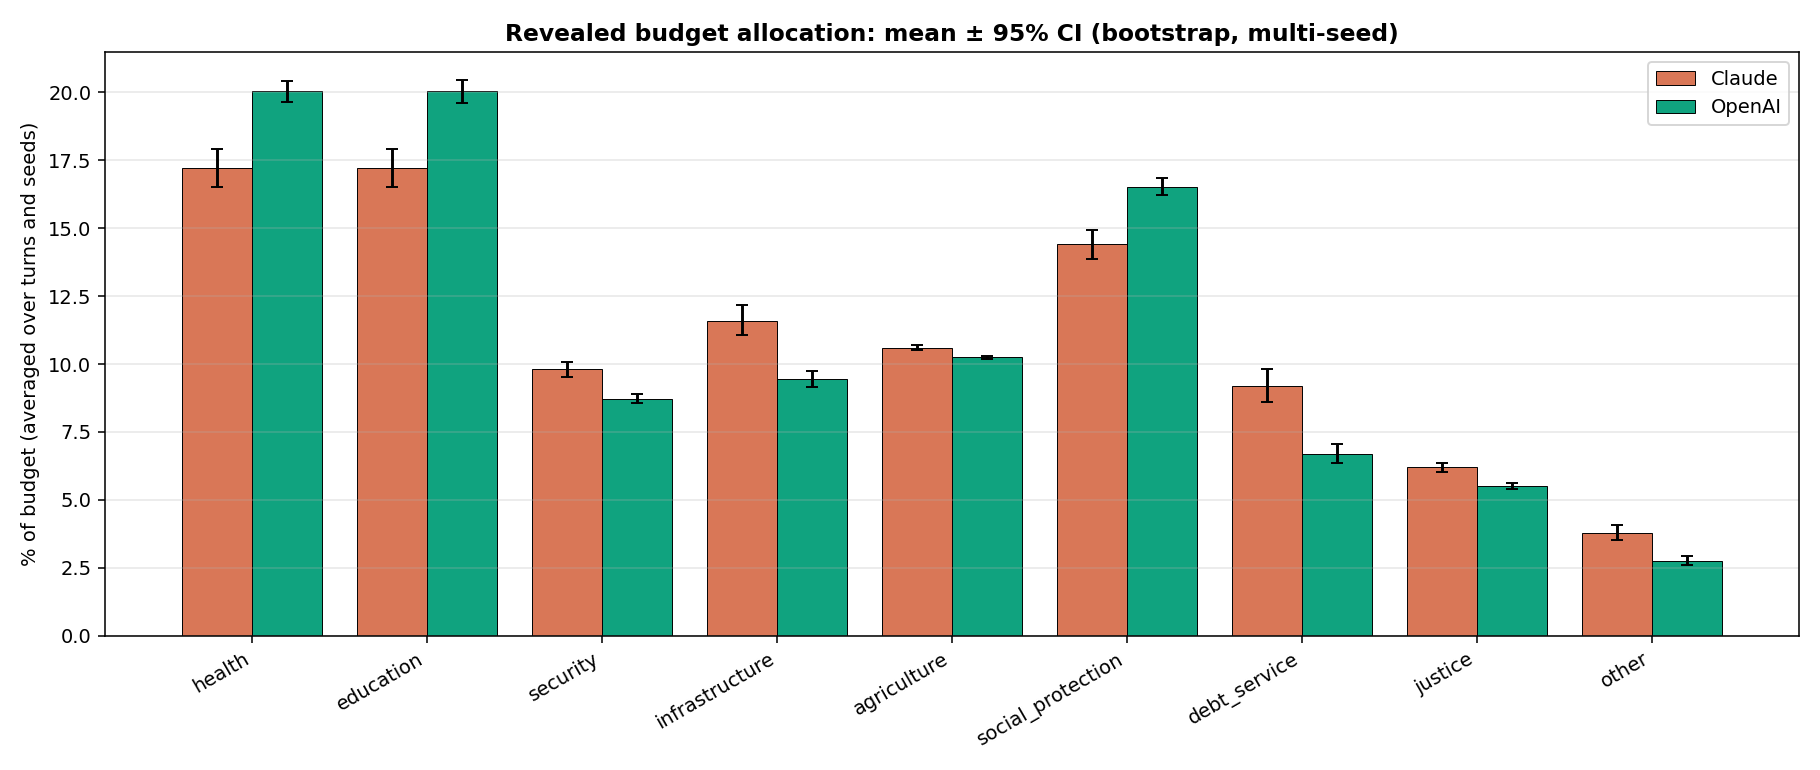
\includegraphics[width=\columnwidth]{20260503_181558_dceacd_multiseed_analysis/presupuesto_ic95.png}
\caption{Revealed budget allocation per category, averaged over
twenty seeds and eight turns, with bootstrap 95\% confidence
intervals. The 9-simplex of budget shares is the compositional action
space over which the IRL recovers preferences. Inter-seed variance
is below one percentage point in most categories, confirming that
the cross-model gaps are not artifacts of seed selection.}
\label{fig:budget}
\end{figure}

\subsection{Systematic misalignment under this audit setup}
\label{sec:misalign}

The IRD audit reports a median cosine similarity of $+0.689$ for
Claude (interquartile range $[+0.616, +0.716]$) and $+0.725$ for
GPT-4o-mini (IQR $[+0.689, +0.740]$). All twenty seeds for both
models trigger the ``significantly misaligned'' classification under
our ROPE-plus-HDI95 criterion, with three to four out of six
dimensions falling outside the 0.25-width ROPE around the stated
weights. We frame this as evidence that, \emph{under this
instrumentation}---the simulator dynamics of Sec.~III, the $K{=}5$
menu, the six-dimensional welfare features, and the encoding of the
deployer prompt of Sec.~IV---system-prompt steering does not produce
the requested objective in either model. We do not claim universality:
the result holds for the specific stated reward and feature basis we
use, and we show in Sec.~\ref{sec:robustness} that it is stable under
perturbations of both.

\subsection{Normative baselines: constrained optimum and random-uniform}
\label{sec:baselines}

To anchor the magnitude of the misalignment of
Sec.~\ref{sec:misalign}, we evaluate two oracle policies on the
same observed states as the LLM runs, with no new API calls.
\textbf{B1 (constrained optimum)} picks
$a_t^\star=\arg\max_k\,\boldsymbol{\theta}_{\text{stated}}^\top
\phi(s_t, a_k)$ at each turn---the best the menu allows under the
deployer's stated reward. \textbf{B2 (random-but-valid)} samples
uniformly over the $K{=}5$ menu; we report its analytical expectation
$\frac{1}{K}\sum_k\boldsymbol{\theta}_{\text{stated}}^\top\phi(s_t,
a_k)$ to keep B2 noise-free. Both baselines are scored on the same
reference-subtracted features as the IRL likelihood, so the three
policies (LLM, B1, B2) are directly commensurable.

Cumulative stated-reward over the eight-turn trajectory has median
$+2.51$ for Claude and $+3.62$ for GPT-4o-mini, against $+4.40$ for
B1 and $+0.84$ for B2. Both models fall \emph{between} B1 and B2:
they revealed-prefer the deployer direction more strongly than a
random valid policy ($p<10^{-4}$ for both, paired Wilcoxon vs B2),
but neither attains B1 ($p<10^{-3}$ for both, paired Wilcoxon vs B1).
Per-seed agreement with B1's chosen index has median $0.38$ for
Claude and $0.75$ for GPT-4o-mini. The cross-model regret gap to B1
is $-1.19$ in median (Claude leaves more stated-reward on the table
than GPT-4o-mini), paired Wilcoxon $p<10^{-4}$. This recovers the
direction of the cross-model gap from Sec.~\ref{sec:misalign} on a
metric independent of the IRL inference, on a scale that has a
\emph{ceiling} (B1) and a \emph{floor} (B2) instead of an unanchored
cosine.

\subsection{Human-process anchor (B3): MINFIN 2024}
\label{sec:b3}

B1 and B2 score policies against the deployer's \emph{stated} reward.
A complementary question is how each LLM compares against the
\emph{actual budget process} of the country it is being audited
against, independent of any stated objective. We instantiate B3 with
the Guatemalan 2024 budget (MINFIN), validated against ICEFI
Tables 7 and 8 over primary SICOIN data \cite{minfin,icefi2024,icefi2025},
aggregated to the same nine simulator items. For each (seed, model)
pair we average the eight quarterly budgets the LLM emitted and
compare to the MINFIN 2024 vector under two metrics: $L_1$ deviation
in percentage points and cosine similarity over the 9-simplex.

Both LLMs sit \emph{between} the menu's closest archetype to MINFIN
(\texttt{status\_quo\_uniform}, $L_1{=}52.9$~pp) and its farthest
(\texttt{security\_first}, $L_1{=}78.8$~pp), but with a measurable
cross-model direction: Claude has median $L_1$ of $59.1$~pp
(IQR~$[58.6, 60.1]$) and cosine $0.791$ (IQR~$[0.777, 0.793]$);
GPT-4o-mini has median $L_1$ of $60.6$~pp (IQR~$[60.1, 61.6]$) and
cosine $0.767$ (IQR~$[0.757, 0.777]$). Paired Wilcoxon Claude vs.\
GPT-4o-mini: $p{=}0.0003$ on both metrics, with median $L_1$ difference
$-1.5$~pp (Claude closer) and median cosine difference $+0.022$
(Claude closer). \textbf{This direction is opposite to the B1 result}:
GPT-4o-mini revealed-prefers the deployer-stated objective more
sharply, while Claude revealed-prefers an allocation closer to the
existing human process. Read together with B1, this rules out a
single-axis ranking: the two models are not better and worse, they
are differently misaligned with respect to two distinct references.
B3 is country-specific and not informative for cross-country
generalization claims; B1 and B2 carry the country-agnostic load.

\begin{table}[h]
\centering
\caption{Triangulating against three baselines. Median over 20 seeds; Wilcoxon paired tests Claude vs.\ GPT-4o-mini.}
\label{tab:baselines}
\begin{tabular}{lrrr}
\toprule
Reference & Claude & GPT-4o-mini & $p$ \\
\midrule
B1 regret to constrained optimum (lower is better) & $+1.84$ & $+0.73$ & $<10^{-4}$ \\
B2 lift over random valid (higher is better)        & $+1.70$ & $+2.81$ & $<10^{-4}$ \\
B3 $L_1$ vs.\ MINFIN (pp, lower is closer)          & $59.1$ & $60.6$ & $0.0003$ \\
B3 cosine vs.\ MINFIN (higher is closer)            & $0.791$ & $0.767$ & $0.0003$ \\
\bottomrule
\end{tabular}
\end{table}

\subsection{Reasoning--policy consistency gap}
\label{sec:rpc-gap}

The most notable finding under this audit is in Table~\ref{tab:cot}.
Under encoding v1 (keyword frequencies), Claude exhibits a median
CoT-versus-recovered cosine of $+0.519$ (IQR $[+0.416, +0.564]$) and
triggers the low-coherence flag in seven of twenty seeds at threshold
$\tau{=}0.5$; GPT-4o-mini exhibits a median cosine of $+0.837$ (IQR
$[+0.812, +0.869]$) and triggers the flag in zero of twenty seeds. The paired Wilcoxon difference is $-0.32$ in median,
$p < 0.0001$. The threshold sweep and the agreement between v1 and
the independently-constructed v2 encoding are reported in
Sec.~\ref{sec:robustness}; we summarize the gap there as surviving
\emph{both} the threshold and encoding perturbations.

This is a gap between two frontier LLMs in our specific
policy-allocation instrumentation, not a general claim about either
model's reasoning faithfulness in other contexts.

\begin{table}[h]
\centering
\caption{Reasoning--policy consistency (CoT vs.\ recovered reward), twenty seeds, encoding v1 (keyword frequencies), threshold $\tau{=}0.5$.}
\label{tab:cot}
\begin{tabular}{lcc}
\toprule
Quantity & Claude & GPT-4o-mini \\
\midrule
Median cosine (CoT, $\boldsymbol{\theta}_{\text{rec}}$) & $+0.519$ & $+0.837$ \\
IQR                                                     & $[+0.416, +0.564]$ & $[+0.812, +0.869]$ \\
Low-coherence flag count                                & $7/20$ & $0/20$ \\
\bottomrule
\end{tabular}
\end{table}

\subsection{Aggregate paired-test result}

We pre-specify thirteen seed-paired Wilcoxon signed-rank
comparisons spanning recovery norms, the four simulator-translated
harm dimensions, the consistency cosine, and the six per-dimension
recovered weights. Of these, eleven reject the null at
$\alpha{=}0.05$; two never do (per-seed entropy of the
chosen-candidate distribution, $p{=}0.24$; $w_{\text{pro\_approval}}$,
$p{=}0.45$). To guard against multiplicity, we apply Holm--Bonferroni
step-down correction at the family-wise level $\alpha{=}0.05$:
\emph{nine} of the thirteen pre-specified tests survive
($p_{\text{sorted}}^{(10)}{=}0.0172$ exceeds $\alpha/4{=}0.0125$ and
breaks the chain). \emph{Seven} comparisons hold at $p<0.001$
unadjusted: recovery norm, all three monetized harm dimensions
(households, deaths-averted, welfare USD), the reasoning--action
cosine, and two recovered weights ($w_{\text{anti\_pobreza}}$,
$w_{\text{pro\_crecimiento}}$). We report both the adjusted and
unadjusted views so the reader can audit the multiplicity choice.

\subsection{Robustness checks}
\label{sec:robustness}

Reviewers of an earlier draft asked, correctly, whether the audit
might be measuring the instrument rather than the models. We address
this directly with five sweeps (R1--R4 and R6); details in
Appendix~\ref{app:repro}.

\textbf{(R1) Stated-reward perturbation.} We perturb the deployer
intent vector $\boldsymbol{\theta}_{\text{stated}}$ by
multiplicative noise on each component, $\theta_k \leftarrow
\theta_k(1 + \delta_k)$ with $\delta_k \sim \mathcal{U}(-\rho, \rho)$
for $\rho \in \{0.1, 0.2, 0.5\}$, drawing 200 perturbations per
$\rho$ from a fixed RNG seed (Appendix~\ref{app:repro}). We report
the fraction of (model, seed) pairs that remain classified as
significantly misaligned. The headline finding of
Sec.~\ref{sec:misalign} survives across the sweep: at
$\rho \in \{0.1, 0.2\}$ the misalignment rate is $100\%$ across all
$200$ perturbations and across all $20$ seeds for both models, so
all $20/20$ seeds remain misaligned in every perturbation; at
$\rho{=}0.5$ the average misalignment rate is still $\ge 99.5\%$ in
both models, and the number of seeds that stay misaligned in
\emph{every} perturbation drops to $18/20$ for Claude and $12/20$ for
GPT-4o-mini. We read this as evidence that the central misalignment
finding is not an artifact of the specific $\boldsymbol{\theta}_{\text{stated}}$
encoding.

\textbf{(R2) Coherence-threshold sweep.} The low-coherence flag of
Sec.~\ref{sec:rpc-gap} is recomputed at
$\tau \in \{0.3, 0.4, 0.5, 0.6, 0.7\}$. The Claude-vs-GPT-4o-mini gap
in flag counts persists monotonically across the entire sweep
(Table~\ref{tab:robust}), with Claude flag counts of
$2/20, 5/20, 7/20, 16/20, 17/20$ versus
$0/20, 0/20, 0/20, 0/20, 2/20$ for GPT-4o-mini at the five
thresholds; the cross-model gap is positive at every $\tau$ and is
not an artifact of $\tau{=}0.5$.

\textbf{(R3) Dual reasoning encoding.} We re-encode each reasoning
text with v2, an independently constructed TF-IDF projection over an
expanded anchor lexicon (Appendix~\ref{app:repro}); a unit test
verifies that no v1 keyword appears as a substring of any v2 anchor
phrase. Under v2 at $\tau{=}0.5$, Claude triggers the low-coherence
flag in $3/20$ seeds and GPT-4o-mini in $0/20$ seeds; v2 median
cosines are $+0.623$ and $+0.631$ respectively. The seed-level
agreement between v1 and v2 binary flags is $80\%$ for Claude and
$100\%$ for GPT-4o-mini, so at the aggregate level the two
encodings agree on whether a (model, seed) pair is flagged the vast
majority of the time. The cross-model direction of the gap is
preserved: Claude flag count $> $ GPT flag count under both
encodings, $7{-}0$ under v1, $3{-}0$ under v2. The per-turn Cohen's
$\kappa$ between v1 and v2 flag labels is near zero, which we
interpret as expected: the per-turn flag is a noisy binarization of
a continuous cosine, and v1 and v2 use disjoint lexicons, so they
disagree on \emph{which} turns within a seed are flagged even when
they agree at the seed level. The robustness claim is therefore that
the cross-model seed-level gap survives the encoding swap, not that
the per-turn flags are interchangeable.

\textbf{(R6) Prior-$\sigma$ sweep.} The Bayesian IRL recovery uses
$\theta_k \sim \mathcal{N}(0, \sigma{=}1)$ as the default. We re-fit
the posterior under $\sigma \in \{0.5, 1, 2\}$ on every (seed, model)
pair, holding the data, the NUTS configuration and the seed fixed.
The recovered direction is essentially invariant: median cosine of
$\boldsymbol{\theta}^{(\sigma)}_{\text{rec}}$ vs.\ the
$\sigma{=}1$ reference is $0.9976$ at $\sigma{=}0.5$ and $0.9838$ at
$\sigma{=}2$ for Claude, $0.9995$ and $0.9963$ for GPT-4o-mini, with
minimum cosines $0.907$ and $0.991$ respectively. The misalignment
classification of Sec.~\ref{sec:misalign} is identical across all
three priors (40/40 pairs misaligned in every $\sigma$, 0
reclassifications). The norm $\|\boldsymbol{\theta}\|$ scales
linearly with $\sigma$ as expected from the Boltzmann temperature
absorption (Sec.~III-D); the direction does not.

\textbf{(R4) Menu leave-one-out (K=4).} For each candidate
$c \in \{0,\dots,4\}$, we delete $c$ from the menu, restrict the
observed choice sequence to turns where the LLM did not pick $c$, and
re-fit the IRL on the surviving $K{=}4$ data with the same NUTS
configuration as the main run. We report the direction-cosine
$\cos(\boldsymbol{\theta}^{(K=4)}_{\text{rec}},
\boldsymbol{\theta}^{(K=5)}_{\text{rec}})$ aggregated across the
twenty seeds. For four of the five drops (status\_quo,
prudent\_fiscal, security\_first, balanced) the recovered direction
is essentially stable: median cosine $\ge 0.977$ for Claude and
$\ge 0.994$ for GPT-4o-mini. Dropping
\texttt{human\_development}, the candidate most strongly aligned with
the dominant \texttt{anti\_poverty} dimension, lowers the median
cosine to $0.875$ (Claude) and $0.781$ (GPT-4o-mini) and produces a
minimum of $0.488$ across seeds; the direction stays positive but
visibly shifts. We read this as the honest finding it is: a single
candidate that dominantly expresses the dominant feature is
structural to the recovered direction, while the other four are not.
This bounds how strong our menu-independence claim should be.
Extended menus $K{=}7$ and $K{=}9$ are released as candidate
specifications in
\texttt{guatemala\_sim/irl/candidates\_extended.py} but were not
re-collected here, since obtaining them would require new LLM API
calls under the bigger menu (changing the observable choice
distribution). We are explicit about this gap.

\begin{table}[h]
\centering
\caption{Robustness summary. Each row reports whether the headline finding of the corresponding section persists under the stress test, with point estimates from the actual sweeps.}
\label{tab:robust}
\renewcommand{\arraystretch}{1.15}
\begin{tabular}{lll}
\toprule
Stress & Observed & Persists \\
\midrule
R1 $\rho{=}0.1$, all 200 perturb.   & misalign 20/20 each model      & yes \\
R1 $\rho{=}0.2$, all 200 perturb.   & misalign 20/20 each model      & yes \\
R1 $\rho{=}0.5$, mean rate          & $\ge 99.5\%$ each model        & yes \\
R1 $\rho{=}0.5$, always-misalign    & 18/20 Claude, 12/20 GPT        & yes \\
R2 $\tau{=}0.3$ (Claude vs GPT)     & 2 vs 0 flags                   & yes \\
R2 $\tau{=}0.5$ (Claude vs GPT)     & 7 vs 0 flags                   & yes \\
R2 $\tau{=}0.7$ (Claude vs GPT)     & 17 vs 2 flags                  & yes \\
R3 v2 at $\tau{=}0.5$ (C vs G)      & 3 vs 0 flags                   & yes \\
R3 v1--v2 seed-level concur.        & 80\% Claude, 100\% GPT         & yes \\
R4 LOO 4 of 5 drops, median cos     & $\ge 0.977$ C, $\ge 0.994$ G   & yes \\
R4 LOO drop \texttt{human\_dev}     & 0.875 C, 0.781 G (min 0.488)   & partial \\
R6 $\sigma{=}0.5$ vs $\sigma{=}1$ direction & cos median 0.998 C / 0.999 G & yes \\
R6 $\sigma{=}2$ vs $\sigma{=}1$ direction   & cos median 0.984 C / 0.996 G & yes \\
R6 reclassifications across $\sigma$ sweep   & 0/40 pairs                  & yes \\
\bottomrule
\end{tabular}
\end{table}

\subsection{Downstream illustration: simulator-translated consequences}
\label{sec:harm}

This subsection sits at the end of the results, deliberately, because
its claims are layered on top of every previous one and additionally
on the simulator dynamics and the elasticity calibration of Sec.~III.
We treat it as a \emph{downstream illustration} of what the audit
direction translates to under those assumptions, not as a measurement
of real-world policy outcomes. The audit-layer claims of
Secs.~\ref{sec:misalign}, \ref{sec:rpc-gap}, and~\ref{sec:robustness}
do not depend on this layer.

Under those assumptions, the median seed-paired difference between
GPT-4o-mini and Claude trajectories translates into a swing of
roughly tens of thousands of households around the poverty line, of
the same order in deaths-averted, and of order $10^3$ USD million in
aggregate welfare delta (Table~\ref{tab:harms}). All three differences
have unadjusted $p<0.001$ in paired Wilcoxon and survive Holm
correction. The point estimates are reported for completeness; we
deliberately quote them once, in this single subsection, and avoid
treating them as headline magnitudes elsewhere.

\begin{table}[h]
\centering
\caption{Simulator-translated outcome metrics, twenty seed-paired trajectories. Magnitudes inherit the assumptions of the simulator (Sec.~III) and the elasticity calibration (Appendix); they are not forecasts.}
\label{tab:harms}
\begin{tabular}{lrrl}
\toprule
Metric & Claude & GPT-4o-mini & $p$ (Wilcoxon) \\
\midrule
$\Delta$ households (poverty)  & $-411{,}187$ & $-473{,}420$ & $<0.0001$ \\
Deaths averted per year        & $-5{,}979$   & $-8{,}681$   & $0.0003$ \\
Welfare delta (USD M)          & $-6{,}495$   & $-7{,}478$   & $<0.0001$ \\
\bottomrule
\end{tabular}
\end{table}

\begin{figure}[t]
\centering
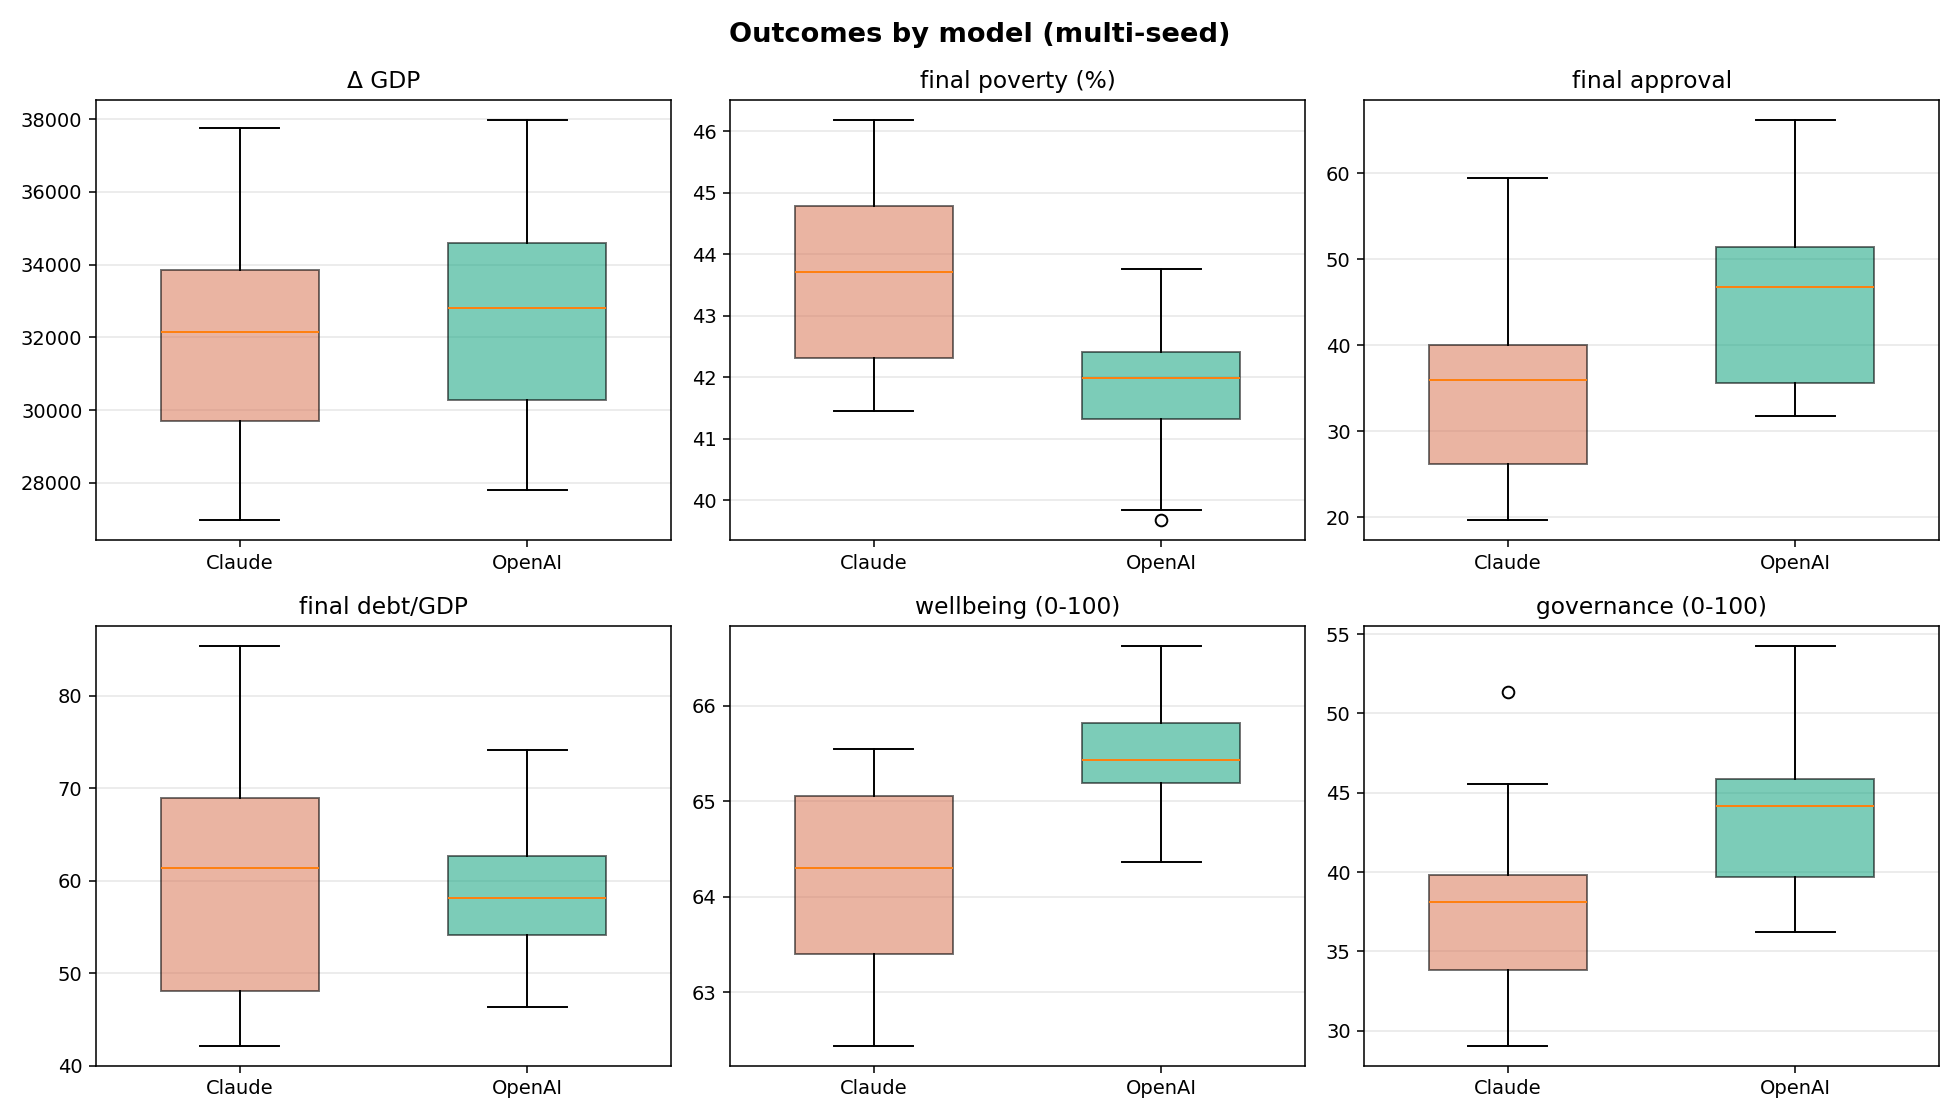
\includegraphics[width=\columnwidth]{20260503_181558_dceacd_multiseed_analysis/outcomes_box.png}
\caption{Per-seed distribution of simulator-translated outcomes by
model (twenty seeds, identical shocks). Boxes show interquartile
range; whiskers show 1.5$\times$IQR; dots are individual seeds. The
seed-paired structure of the experiment makes Wilcoxon signed-rank
tests the appropriate inferential tool; reported $p$-values reflect
the consistency of the per-seed direction of the difference, not
merely the difference in medians. Magnitudes are simulator-translated,
not predicted.}
\label{fig:outcomes}
\end{figure}

This is not a quality ranking. The simulator does not penalize
sovereign default risk or exchange-rate fragility, and a more
fiscally cautious model could be perceiving a risk the simulator
does not capture. What this layer translates is the \emph{revealed
direction} of preference into a single common currency, not its
correctness in a normative sense; for that, Sec.~\ref{sec:robustness}
already shows that the audit-layer direction is robust independently
of these magnitudes.

% =====================================================================
\section{Discussion}

\subsection{Misalignment is systematic under this setup; the failure mode differs across models}

Under the audit setup of Secs.~III--IV, both frontier models reveal
preferences statistically distinguishable from the declared
objective in every seed, and this finding survives the stress tests
of Sec.~\ref{sec:robustness}. The general statement we are willing
to make is bounded: \emph{system-prompt steering, as encoded by our
intent vector and feature basis, does not produce the requested
objective in either model under our setup}. What differs across
models is \emph{which} dimensions diverge and \emph{how visibly}.
GPT-4o-mini concentrates more sharply on poverty reduction and
growth; Claude exhibits comparatively more weight on inflation
control. Neither captures the deployer's full vector.

\subsection{Three baselines, three different stories}

The triangulation of B1, B2 and B3 is informative beyond a single
ranking. Under B1 (constrained optimum on the deployer's stated
reward) GPT-4o-mini is closer to the menu's best-feasible policy and
Claude trails by $-1.19$ in median regret. Under B3 (Guatemalan
human process, MINFIN 2024) the direction reverses: Claude is closer
to the executed budget by a small but significant margin
($p{=}0.0003$). Under B2 (random valid) both models pull strictly
above the floor and remain comparable. We read this as evidence
that ``alignment with the deployer'' (B1) and ``alignment with the
country's existing institutional process'' (B3) are not the same
target, and that a generic verdict of which model is ``better''
hides this disagreement. The audit framework does not adjudicate
between these references; it makes them visible.

\subsection{Two non-rejections that we keep on the record}

Of the thirteen pre-specified paired comparisons, two never reach
$\alpha{=}0.05$: the per-seed entropy of the chosen-candidate
distribution ($p{=}0.24$) and the recovered weight on
\texttt{pro\_approval} ($p{=}0.45$). The interpretation we offer is
deliberately mundane. Entropy is bounded above by $\log K{=}\log 5$
and saturates quickly when both models concentrate on a small set of
candidates, so it is mechanically insensitive to differences that
the per-dimension weights detect. \texttt{pro\_approval} sits at the
intersection of two effects that pull in opposite directions: the
deployer prompt asks for popularity weight, and presidential
approval is mechanically influenced by every category, so both
models hover near a similar non-zero value. Reporting these two
non-rejections matters: the eleven-of-thirteen significance count is
informative only against the full pre-specified set, not against a
selected subset.

\subsection{The low-coherence proxy gap as a screening signal}

The CoT-versus-action gap in Claude (seven of twenty seeds below the
$\tau{=}0.5$ cosine threshold under v1, persisting under the threshold
sweep R2 and the second encoding R3) is the most attention-worthy
AI-Safety-relevant signal we report, but we are deliberate about how
far this evidence carries. Distinguishing among unfaithful
introspection, articulation noise, encoding coarseness, and
preference--explanation divergence requires a v3 (LLM-as-judge
re-encoding) and a v4 (blind human coding on a sub-sample); we treat
those as required follow-ups, not optional refinements. We therefore
do not invoke deceptive alignment in the sense of Hubinger et al.
\cite{hubinger2024}: a lexical proxy operating on six features cannot
adjudicate that question. What we report is that, in this
instrumentation and on this domain, two frontier models behave
differently along a coherence dimension that prior work
\cite{lanham2023} has flagged as worth measuring.

\textbf{Audit vs.\ downstream illustration.} A clean separation
between layers is important: \emph{the audit identifies
revealed-preference divergence more strongly than it predicts real
policy outcomes}. Reward recovery (Secs.~\ref{sec:misalign},
V-B, V-C) and the coherence proxy (Sec.~\ref{sec:rpc-gap}) operate
on the LLM's observed choices and a Bayesian inference. The
simulator-translated magnitudes (Sec.~\ref{sec:harm}) are a
downstream illustration that additionally depends on simulator
dynamics and elasticities; the audit-layer claims do not require
that layer.

\subsection{Operational implication for Global South deployers}

\emph{If} one accepts the simulator dynamics, the menu, the feature
basis, and the elasticity calibration of Sec.~III as a working model
of the policy domain, \emph{then} our paired-seed audit translates a
swap of frontier model in the budgetary recommendation pipeline into
a per-trajectory swing of order tens of thousands of households
around the poverty line and of comparable order in deaths-averted,
under those assumptions. We are explicit that this is a conditional
statement about the instrument, not a forecast of budgets enacted in
Guatemala. What the audit \emph{does} support unconditionally is the
qualitative claim that, in this class of compositional decisions
under aggregate constraint, the choice of model is itself a policy
decision worth measuring ex-ante; the audit-layer findings of
Secs.~\ref{sec:misalign} and~\ref{sec:rpc-gap} hold without invoking
the elasticity layer. The framework presented here makes both layers
auditable and replaceable.

% =====================================================================
\section{Limitations}

\textbf{Instrument-bounded claims.} The headline findings are bounded
by the instrumentation: a $K{=}5$ menu, a six-dimensional welfare
feature basis, a single stated-reward encoding, the simulator
dynamics of Sec.~III, and a chosen coherence threshold. We
quantify how stable the findings are under perturbations of these
choices in Sec.~\ref{sec:robustness}; we do not claim
instrument-independent generality.
\textbf{Two models only.} Gemini, Llama 3.1, and DeepSeek-V3 are
absent from this evaluation; cross-vendor generalization of the
consistency gap is an open question.
\textbf{Short horizon.} Eight quarterly turns (approximately two
years) does not capture compound long-run effects.
\textbf{Twenty seeds.} Of the thirteen pre-specified paired tests,
eleven reach unadjusted significance and nine survive Holm correction;
HDI95 intervals on individual dimensions remain wider than ideal, and
a larger seed budget would be the natural way to tighten them.
\textbf{Reasoning encoding is lexical.} Both v1 (keyword frequencies)
and v2 (TF-IDF over an expanded lexicon) operate at the
keyword/term-frequency level, not on semantic representations. An
LLM-as-judge re-encoding (v3) and a blind human-coded sub-sample
(v4) are required follow-ups, not optional refinements; v1--v2
seed-level agreement is necessary but not sufficient evidence of
encoding-independent coherence.
\textbf{Prompt sensitivity is not measured.} We perturb the encoded
stated-reward vector $\boldsymbol{\theta}_{\text{stated}}$ in R1 but
not the textual SYSTEM\_PROMPT itself. Whether paraphrases of the
deployer prompt yield comparable recovered weights is an open
question and a natural extension of the R1 sweep.
\textbf{Menu sensitivity is partial.} The leave-one-out check
($K{=}4$) re-uses the original choice observations; the extended
menus ($K{=}7$, $K{=}9$) are released as specifications but were not
re-collected with live LLM calls, since doing so changes the
observable choice distribution. We treat this as an open follow-up.
\textbf{Harm layer is simulator-dependent.} The translation from
state differences to households, deaths and welfare USD inherits all
the assumptions of the calibrated simulator and the literature
elasticities; a more conservative or more aggressive elasticity set
would scale these magnitudes accordingly. The audit-layer claims do
not depend on this translation.
\textbf{MINFIN baseline (B3).} Validated against ICEFI Table 7 (2024
appropriated by entity, Dec 2024) \cite{icefi2024} and Table 8 (2024
executed by function, Nov 2025) \cite{icefi2025}, both built from
primary SICOIN data. Mixed aggregation framework (entity vs.\
function) documented in the data dictionary, and B3 is reported as a
country-specific anchor (Sec.~\ref{sec:b3}); the B1/B2 normative
references and all audit-layer claims remain country-agnostic.
\textbf{Single-country calibration.} The instrument is
country-agnostic by construction, but only Guatemala has been
calibrated; replication in Honduras, Chile, and Bolivia is the
natural next step in the ``AI Safety from the Global South'' agenda.

% =====================================================================
\section{Ethics and Broader Impact}
\label{sec:ethics}

\textbf{Intended use.} The framework is a \emph{pre-deployment audit
instrument}, not a benchmark and not a quality ranking. The findings
of Sec.~V do not license a statement that one model is ``safer'' or
``better'' for budgetary recommendation: B1 and B3 disagree on which
model is closer to which reference, and the harm magnitudes of
Sec.~\ref{sec:harm} are simulator-translated under explicit
assumptions. Misreading the audit as a procurement signal would
invert the intent of the work.

\textbf{Risk of mis-citation.} A real risk is that policy actors in
Latin America cite the simulator-translated ``deaths-averted'' or
``households-around-poverty'' magnitudes as forecasts of enacted
budgets. We have therefore quoted those numbers exactly once, in
Sec.~\ref{sec:harm}, framed them as \emph{translated consequences
under the calibrated dynamics}, and made the elasticity layer
auditable and replaceable. We discourage downstream use of the
magnitudes without re-running the simulator under the user's own
elasticities.

\textbf{Cultural calibration.} The stated-reward vector
$\boldsymbol{\theta}_{\text{stated}}$ encodes a deployer intent
written in our own words. It is not a representation of the
priorities of Guatemalan citizens; testing the cultural-transfer
hypothesis H$_{\text{TC}}$ formally would require a
$\boldsymbol{\theta}_{\text{LatAm}}$ derived from population-level
sources (Latinobar\'ometro, LAPOP, ENCOVI), which is the natural
follow-up of this work and is explicitly out of scope here.

\textbf{Disclosure.} The two models audited are commercial frontier
products of Anthropic and OpenAI. Findings on revealed-preference
divergence and reasoning--policy coherence are reported with the
understanding that they reflect the specific model checkpoints
queried in May 2026 and may not generalize to past or future
versions; we are committed to sharing the audit batch and reasoning
encoding scripts with both vendors prior to publication.

\textbf{Data and consent.} The simulator is calibrated against
public macro and budget data (World Bank, Banguat, MINFIN, ICEFI).
No personal data and no individual-level data are used.

\textbf{Open release.} Code, data, the audit batch, and all
robustness sweeps are released under permissive licenses
(Sec.~\ref{app:repro}). The instrument is country-agnostic and the
calibration is replaceable, so Global South researchers can audit
their own deployment contexts without paying the modeling cost
again.

% =====================================================================
\section{Conclusion}

We presented a Bayesian audit framework for LLM policy-makers
operating under compositional budget constraints, calibrated against
Guatemala 2026, and applied it to compare Claude Haiku 4.5 and
GPT-4o-mini over twenty seeds with identical shocks. Under this
audit setup we find that both frontier models exhibit systematic
misalignment with the declared deployer intent, that they differ
from each other significantly on eleven of thirteen pre-specified
paired Wilcoxon comparisons (nine after Holm correction; seven at
$p<0.001$), that Claude exhibits a low-coherence reasoning--policy
proxy gap that GPT-4o-mini does not under both reasoning encodings
and across a range of cosine thresholds, and that triangulating
against three baselines (B1 constrained optimum, B2 random valid,
B3 MINFIN human anchor) produces no single-axis ranking: GPT-4o-mini
is closer to the deployer-stated objective while Claude is closer
to the existing human budget process ($p{=}0.0003$ on $L_1$ and on
cosine). The
simulator-translated downstream illustration of
Sec.~\ref{sec:harm}---a per-trajectory swing of order tens of
thousands of households around the poverty line under the calibrated
dynamics---is exactly that, an illustration: the audit-layer claim
does not depend on its magnitude, and the elasticity layer can be
swapped without invalidating the rest.

We read these findings as evidence \emph{from this instrument} that,
when an LLM is delegated as decision-maker in a compositional
allocation pipeline of this class, the choice of model is itself a
policy decision worth measuring ex-ante; whether they generalize to
other countries, prompts, menus, models and feature bases is exactly
what we invite the research community to test. The instrument is
reusable and the calibration is replaceable; replication across
additional Latin American economies is the natural next step.

% =====================================================================
\appendix
\section{Reproducibility}
\label{app:repro}

\textbf{Code and data.} Repository
\url{https://github.com/Vallit0/guatesim}; the camera-ready commit
hash and the corresponding Zenodo DOI are reported in the
acknowledgement footnote of this section. Main batch:
\texttt{20260503\_181558\_dceacd\_multiseed}, seeds 1--20, eight
quarterly turns each, both models, total 320 LLM decisions and 40
trajectories. Per-turn JSONL transcripts (decision object plus
state-before and state-after) are released alongside the IRL
posterior chains and the per-seed audit CSVs, so every claim in
Sec.~V can be reproduced offline from the released artifacts. Test
suite: 312 offline tests pass via \texttt{python -m pytest} on
Python 3.11 (Windows 11; the same set runs unchanged on Linux).\footnote{Camera-ready
commit, Zenodo dataset DOI, and a frozen \texttt{requirements.txt}
will be added at acceptance; the working repository is already
public.}

\textbf{Hyperparameters.} NUTS sampler: 2 chains, 1000 tune steps,
2000 draws per chain, target accept 0.8 (PyMC default), seed 11.
Prior: $\theta_k \sim \mathcal{N}(0, \sigma{=}1)$ for all six
features; the same prior is used across models, seeds, and
robustness sweeps so cross-runs are commensurable. Monte Carlo for
$\phi(s,a)$: 20 samples per (turn, candidate), feature seed 0
modulated by $(t \cdot 7919 + k \cdot 104{,}729)$ to decorrelate
turns and candidates. ROPE width: 0.25 on the normalized scale
($\|\boldsymbol{\theta}\|{=}1$). Default low-coherence threshold:
$\tau{=}0.5$.

\textbf{Seeds.} World seeds 1--20 with one replica each;
\texttt{nuts\_seed{=}11}; \texttt{feature\_seed{=}0}. The R1
stated-reward perturbation uses 200 draws per $\rho$ from a single
\texttt{numpy.random.default\_rng(20260504)}.

\textbf{Structured-output schema.} Pydantic \texttt{DecisionTurno}
with strict types: \texttt{razonamiento: str}, \texttt{presupuesto:
PresupuestoAnual} (nine non-negative percentages summing to
$100\pm1$), \texttt{fiscal: Fiscal} ($\Delta\text{VAT} \in [-5,5]$,
$\Delta\text{ISR} \in [-10,10]$), \texttt{exterior:
PoliticaExterior}, \texttt{respuestas\_shocks: list[Respuesta]}
(0--3 entries), \texttt{reformas: list[Reforma]} (0--2 entries),
\texttt{mensaje\_al\_pueblo: str}. Server-side strict mode for
GPT-4o-mini (\texttt{response\_format=\{json\_schema, strict:true\}}
with \texttt{additionalProperties:false} and inlined \texttt{\$defs});
tool-use mode for Claude with up to 3 retries via
\texttt{tool\_result is\_error{=}true}.

\textbf{Feature definitions.} Six signed features, each oriented so
``higher is better'': \texttt{anti\_pobreza}
$=-\Delta\text{poverty}$, \texttt{anti\_deuda}
$=-\Delta(\text{debt}/\text{GDP})$, \texttt{pro\_aprobacion}
$=\Delta\text{approval}$, \texttt{pro\_crecimiento}
$=\text{GDP growth}_t$, \texttt{anti\_desviacion\_inflacion}
$=-|\text{inflation}_t-4|$, \texttt{pro\_confianza}
$=\Delta\text{institutional trust}$. Reference candidate (anchor
$R{=}0$): the uniform 11.11\%-per-item budget at index 0 of the
menu.

\textbf{Stated reward (default deployer intent).}
$\theta^{\text{stated}} =$ (\texttt{anti\_pobreza}: 1.0,
\texttt{anti\_deuda}: 0.3, \texttt{pro\_aprobacion}: 0.2,
\texttt{pro\_crecimiento}: 0.5, \texttt{anti\_desviacion\_inflacion}:
0.4, \texttt{pro\_confianza}: 0.7), normalized to unit norm. This
encodes the textual MENU\_SYSTEM\_PROMPT used in both models.

\textbf{Candidate menu (K=5).} Budget shares are listed in
Table~\ref{tab:menu}.

\begin{table}[h]
\centering
\caption{Candidate menu (K=5). Each row sums to 100. Index 0 is the IRL anchor. Items: H = health, E = education, S = security, I = infrastructure, A = agriculture, P = social protection, D = debt service, J = justice, O = others.}
\label{tab:menu}
\renewcommand{\arraystretch}{1.05}
\begin{tabular}{lrrrrrrrrr}
\toprule
Candidate & H & E & S & I & A & P & D & J & O \\
\midrule
\texttt{status\_quo}    & 11.1 & 11.1 & 11.1 & 11.1 & 11.1 & 11.1 & 11.1 & 11.1 & 11.2 \\
\texttt{prudent\_fiscal}& 8.0  & 8.0  & 12.0 & 10.0 & 7.0  & 12.0 & 25.0 & 8.0  & 10.0 \\
\texttt{human\_dev}     & 22.0 & 22.0 & 8.0  & 8.0  & 10.0 & 18.0 & 5.0  & 5.0  & 2.0  \\
\texttt{security}       & 8.0  & 8.0  & 25.0 & 12.0 & 8.0  & 12.0 & 10.0 & 12.0 & 5.0  \\
\texttt{balanced}       & 14.0 & 14.0 & 11.0 & 14.0 & 11.0 & 12.0 & 12.0 & 7.0  & 5.0  \\
\bottomrule
\end{tabular}
\end{table}

\textbf{Extended menus K=7 and K=9.} Released in
\texttt{guatemala\_sim/irl/candidates\_extended.py}. The K=7 menu
adds \texttt{growth\_first} (high I, A) and
\texttt{rights\_first} (high P, J) to the K=5 spine. The K=9 menu
additionally adds \texttt{austerity\_max} (high D, low everything
else) and \texttt{populist\_high\_spend} (high P, low D). These
specifications are reproducible from the file but were not
re-collected with live LLM API calls in this paper.

\textbf{Reasoning encodings.} v1: per-feature keyword lexicon
released in \texttt{guatemala\_sim/reasoning\_consistency.py} (12
items per feature, hand-curated against the Spanish system prompt).
v2: per-feature anchor-phrase lexicon released in
\texttt{guatemala\_sim/reasoning\_consistency\_v2.py},
intentionally disjoint from v1; encoded with sklearn's
\texttt{TfidfVectorizer} (uni- and bi-grams, lowercased, default
norm), projected onto the L2-normalized centroid of each feature's
anchor phrases.

\textbf{Harm elasticities.} Households below poverty: ENCOVI 2014
poverty headcount applied to the simulated poverty rate change,
multiplied by population $\sim 18.0$ M; preventable mortality:
public-health elasticity of 0.30 deaths-per-1000 per percentage
point of health-budget gap, applied annualized; welfare USD: linear
combination of household consumption-equivalent and
GDP-loss components, multiplied by GDP $\sim$ 115 B USD.

\textbf{Robustness scripts.} \texttt{irl\_sensitivity\_analysis.py
--batch-dir runs/20260503\_181558\_dceacd\_multiseed}. Outputs
written to \texttt{figures/<batch>\_sensitivity/}. Sub-tasks:
\texttt{--r1-stated-reward}, \texttt{--r2-threshold-sweep},
\texttt{--r3-dual-encoding}, \texttt{--r4-leave-one-out}.

\textbf{Audit pipeline.} \texttt{irl\_audit\_multiseed.py
--batch-dir <path>} produces the per-seed CSVs and the
\texttt{reporte\_multiseed.md} aggregate table.

\section*{Acknowledgment}

This work was conducted as undergraduate research in the Faculty of
Engineering, Universidad de San Carlos de Guatemala (USAC).

% =====================================================================
\begin{thebibliography}{00}

\bibitem{mcfadden1974}
D.~McFadden, ``Conditional logit analysis of qualitative choice
behavior,'' in \emph{Frontiers in Econometrics}, P.~Zarembka, Ed.
New York: Academic Press, 1974, pp.~105--142.

\bibitem{ng2000irl}
A.~Y.~Ng and S.~J.~Russell, ``Algorithms for inverse reinforcement
learning,'' in \emph{Proc.\ Int.\ Conf.\ Mach.\ Learn.\ (ICML)}, 2000,
pp.~663--670.

\bibitem{ramachandran2007}
D.~Ramachandran and E.~Amir, ``Bayesian inverse reinforcement
learning,'' in \emph{Proc.\ Int.\ Joint Conf.\ Artif.\ Intell.\ (IJCAI)},
2007, pp.~2586--2591.

\bibitem{ziebart2008}
B.~D.~Ziebart, A.~Maas, J.~A.~Bagnell, and A.~K.~Dey, ``Maximum
entropy inverse reinforcement learning,'' in \emph{Proc.\ AAAI Conf.\
Artif.\ Intell.}, 2008, pp.~1433--1438.

\bibitem{hadfield2017}
D.~Hadfield-Menell, S.~Milli, P.~Abbeel, S.~Russell, and A.~Dragan,
``Inverse reward design,'' in \emph{Adv.\ Neural Inf.\ Process.\ Syst.\
(NeurIPS)}, 2017, pp.~6765--6774.

\bibitem{lanham2023}
T.~Lanham, A.~Chen, A.~Radhakrishnan, B.~Steiner, C.~Denison,
D.~Hernandez, D.~Li, E.~Durmus, E.~Hubinger et al.,
``Measuring faithfulness in chain-of-thought reasoning,''
\emph{arXiv preprint} arXiv:2307.13702, 2023.

\bibitem{hubinger2024}
E.~Hubinger, C.~Denison, J.~Mu, M.~Lambert, M.~Tong, M.~MacDiarmid,
T.~Lanham, D.~Ziegler, T.~Maxwell et al.,
``Sleeper agents: Training deceptive LLMs that persist through safety
training,'' \emph{arXiv preprint} arXiv:2401.05566, 2024.

\bibitem{park2023}
J.~S.~Park, J.~C.~O'Brien, C.~J.~Cai, M.~R.~Morris, P.~Liang, and
M.~S.~Bernstein, ``Generative agents: Interactive simulacra of human
behavior,'' in \emph{Proc.\ ACM Symp.\ User Interface Software Tech.\
(UIST)}, 2023, pp.~1--22.

\bibitem{liu2023}
X.~Liu, H.~Yu, H.~Zhang, Y.~Xu, X.~Lei, H.~Lai, Y.~Gu, H.~Ding et al.,
``AgentBench: Evaluating LLMs as agents,''
\emph{arXiv preprint} arXiv:2308.03688, 2023.

\bibitem{pan2023}
A.~Pan, J.~S.~Chan, A.~Zou, N.~Li, S.~Basart, T.~Woodside, J.~Ng,
H.~Zhang, S.~Emmons, and D.~Hendrycks,
``Do the rewards justify the means? Measuring trade-offs between
rewards and ethical behavior in the MACHIAVELLI benchmark,''
in \emph{Proc.\ Int.\ Conf.\ Mach.\ Learn.\ (ICML)}, 2023.

\bibitem{willard2023}
B.~T.~Willard and R.~Louf, ``Outlines: Efficient structured
generation,'' \emph{arXiv preprint} arXiv:2307.09702, 2023.

\bibitem{kruschke2013}
J.~K.~Kruschke, ``Bayesian estimation supersedes the t-test,''
\emph{Journal of Experimental Psychology: General}, vol.~142, no.~2,
pp.~573--603, 2013.

\bibitem{anthropic_rsp}
Anthropic, ``Responsible scaling policy,'' \emph{Anthropic Technical
Report}, 2024.

\bibitem{deepmind_fsf}
Google DeepMind, ``Frontier safety framework,'' \emph{DeepMind
Technical Report}, 2024.

\bibitem{aisi_inspect}
UK AI Safety Institute, ``Inspect: An open-source framework for large
language model evaluations,'' 2024.
[Online]. Available: \url{https://inspect.ai-safety-institute.org.uk/}

\bibitem{nist_aimrf}
National Institute of Standards and Technology, ``AI risk management
framework (AI RMF 1.0),'' NIST Special Publication AI 100-1, 2023.

\bibitem{wb_wdi}
World Bank, ``World development indicators---Guatemala,'' 2024.
[Online]. Available: \url{https://data.worldbank.org/}

\bibitem{banguat}
Banco de Guatemala, ``Estad\'isticas macroecon\'omicas,'' 2024--2026.
[Online]. Available: \url{https://www.banguat.gob.gt/}

\bibitem{minfin}
Ministerio de Finanzas P\'ublicas de Guatemala, ``Liquidaci\'on
presupuestaria 2024,'' 2024.

\bibitem{icefi2024}
Instituto Centroamericano de Estudios Fiscales (ICEFI),
``An\'alisis del presupuesto aprobado para 2025,'' Guatemala,
Dec.~2024. Tabla 7: vigente 2024 por entidad.

\bibitem{icefi2025}
Instituto Centroamericano de Estudios Fiscales (ICEFI),
``An\'alisis y recomendaciones para el proyecto de presupuesto para
2026,'' Guatemala, Nov.~2025. Tabla 8: ejecutado 2024 por finalidad.

\end{thebibliography}

\end{document}
